% İskelet: IJCV (Springer sn-jnl) şablonuna geçirilecek; burada genel article sınıfı kullanıldı. Metin kaynağı: paper/draft.md.
% Metin: paper/body.tex (scripts/md2tex.py ile draft.md'den üretilir; elle düzenlemeyin). Derleme: pdflatex+bibtex (Overleaf'te de çalışır).
\documentclass[11pt]{article}
\usepackage[a4paper,margin=2.5cm]{geometry}
\usepackage[utf8]{inputenc}
\usepackage[T1]{fontenc}
\usepackage{booktabs,graphicx,amsmath,amssymb,hyperref,longtable,array,calc,float}
\usepackage[numbers]{natbib}
\providecommand{\tightlist}{\setlength{\itemsep}{0pt}\setlength{\parskip}{0pt}}
\title{When Does Expert Routing Matter? Multi-Criteria and Reinforcement-Learned Routing\\in Two Vision-Language MoE Models}
\author{}
\begin{document}
\maketitle
\begin{abstract}Sparse Mixture-of-Experts (MoE) vision-language models route each token to a few experts, and many proposals promise smarter routers. We test the premise that routing carries exploitable signal, on two frozen backbones and one 8 GB GPU, with DecisionMoE: a router that ranks experts with TOPSIS and lets a PPO policy choose criterion weights and the number of active experts K per step, compared with the gate's Top-K at matched, token-weighted expert FLOPs. (i) On a sparsely upcycled model (MoE-LLaVA-Phi2-2.7B$\times$4, 8,803 synthetic questions, POPE) accuracy is insensitive to expert selection: Top-K for K=1..4, random routing, single experts and fixed MCDM routing all fall in a 2.5-point band, and a learned policy only rediscovers K=1. (ii) On a model with 64 natively trained experts (DeepSeek-VL2-Tiny) the picture reverses: random experts give 0.000 accuracy and dropping the best expert costs 8.8 points, yet Top-3 is within 0.8 points of Top-6 at half the FLOPs. TOPSIS re-ranking adds nothing, even with an oracle domain label. (iii) Adaptive K helps in at most one of three long-generation tasks. With brief chain-of-thought on AI2D, ScienceQA-IMG and A-OKVQA, retrained PPO policies ($\lambda$=0.4) beat the matched-FLOPs Top-K mixture on AI2D (+1 to +2 points) and ScienceQA-IMG (+1 to +9), but a static asymmetric rule (small K in prefill, larger in decode) explains the AI2D gain, and on A-OKVQA the policies merely rediscover Top-3 or Top-2 (−0.9 to −0.1 points against the best static/Top-K hull, CIs include 0). Only on ScienceQA-IMG do the policies keep +1 to +8 points over that hull (four of five seeds with CIs excluding 0), by choosing K per question; they do not transfer across datasets and are unstable at stronger cost pressure. (iv) A step-averaged FLOPs reward is gamed by the policy (reported 0.33, true token-weighted 0.99), and 7.5\% of benchmark references are wrong, with 44\% of flagged hallucinations being broken traps.
Routing matters when experts are diverse, but beyond the gate's Top-K the achievable gain is small; we recommend reporting sensitivity analyses and token-weighted costs.
\end{abstract}% draft.md Abstract bölümünden
\section{Introduction}\label{introduction}

Sparse Mixture-of-Experts (MoE) vision-language models activate a fixed number of experts per token. Prefill over hundreds of image tokens dominates the cost, yet questions differ widely in how much expert capacity they need: on a multiple-choice science benchmark the same model loses about 19 points when K drops from 3 to 2, while on a knowledge-based benchmark K=3 is almost as accurate as K=6. A router that adapts K to the question could trade accuracy for compute where it is cheap to do so. Existing adaptive-routing work trains such routers inside the model; we ask what can be achieved on a \emph{frozen} model without touching the gate, and how to tell a real gain from an artefact.

We make two contributions on one 8 GB GPU. First, \textbf{DecisionMoE-K}, a PPO policy that selects the number of active experts for the prefill and for every decoded token under a token-weighted routed-expert FLOPs budget; we test it with and without TOPSIS ranking of the experts. Second, a \textbf{matched-cost evaluation protocol} that we find necessary: (a) cost is token-weighted (a step-averaged reward is exploited by the policy), (b) policies are compared at equal FLOPs against the upper convex hull of uniform Top-K \emph{and} static asymmetric rules, and (c) every policy is trained with several seeds and evaluated once on a held-out test set with paired bootstrap intervals.

Contributions.
1. \textbf{DecisionMoE-K.} A budget-aware per-question, per-step K policy for frozen MoE-VLMs (§3). With $\lambda$=0.4 it is never significantly worse than the best static or Top-K reference on three tasks (11 seeds) and significantly better where the accuracy-vs-K curve has a cliff (ScienceQA-IMG: +1 to +8 points over the hull; 14--22\% fewer FLOPs than Top-3 at 1--4 points lower accuracy), §5.2.
2. \textbf{A matched-cost protocol with static references}, which shows that the apparent AI2D gain (+1 to +2 points over uniform Top-K) is fully explained by a static asymmetric rule, and that on A-OKVQA the policy only rediscovers Top-3/Top-2 (§5.2).
3. \textbf{TOPSIS does not help.} MCDM re-ranking of the gate's experts adds no accuracy on two backbones, even with an oracle domain label, because its informative criteria are what the gate already encodes (§5.6, §5.4). Routing choice is irrelevant on an upcycled model and decisive but already near-optimal on a natively trained one (§5.6, §5.3).
4. \textbf{Reward-hacking case study.} A step-averaged FLOPs reward is exploited (reported 0.33, true 0.99); a token-weighted reward fixes it (§5.1).
5. \textbf{Benchmark audit.} 7.5\% of references in our synthetic benchmark are wrong and 44\% of flagged hallucinations are broken traps (§5.7); negative pilots (expert pools, token-level top-p) are reported rather than discarded (§5.3, §5.5).

\section{Related work}\label{related-work}

\textbf{Sparse upcycling and MoE VLMs.} Sparse upcycling \citep{komatsuzaki2023upcycling} initialises every expert from one dense feed-forward block; MoE-LLaVA \citep{lin2024moellava} applies it to a vision-language model. DeRS \citep{huang2025ders} and related analyses show that upcycled experts remain close in weight space, which is consistent with our finding that their selection is irrelevant. DeepSeek-VL2 \citep{wu2024deepseekvl2} instead trains fine-grained experts natively.
\textbf{Adaptive and learned routing.} Ada-K \citep{yue2025adak} and related work vary the number of active experts per token, in some cases with reinforcement learning. We differ by comparing against the gate's Top-K at matched token-weighted cost on a frozen model and by reporting where such policies fail.
\textbf{MCDM.} TOPSIS \citep{hwang1981madm} ranks alternatives by closeness to an ideal solution over weighted criteria; we use it as an expert ranker.
\textbf{Evaluation pitfalls.} POPE \citep{li2023pope} measures object hallucination; reward misspecification and gaming \citep{skalse2022reward, amodei2016concrete} motivate our reward-hacking analysis; the policy is trained with PPO and GAE \citep{schulman2017ppo, schulman2016gae}.

\section{Method}\label{method}

\textbf{Routing interface.} Both backbones are frozen and nf4-quantised. A router replaces the gate decision at every MoE layer. One decision per generation step (prefill is one step, each decoded token another) is shared by all layers. The cost measure is the \textbf{token-weighted fraction of routed-expert FLOPs}, K/K\_max averaged over tokens, so the $\approx$600-token prefill dominates (this is what the step-averaged reward got wrong, §5.1).

\textbf{TOPSIS expert ranking.} For each candidate expert a decision matrix of criteria is built, normalised, weighted and scored by closeness to the ideal solution; the top-K by closeness are selected and their gate probabilities renormalised. On MoE-LLaVA (4 experts) the seven criteria are task utility, modality match, specialisation, reliability, latency, FLOPs share and load (reliability and latency are constant tables; \texttt{DEVIATIONS.md} C1--C2). On DeepSeek-VL2-Tiny (64 experts) the criteria are gate probability, a domain prior (train usage share, given by an oracle domain label), specialisation and load.

\textbf{DecisionMoE-K (PPO policy).} On MoE-LLaVA the state (dim 78) comprises a projected hidden state, modality, entropy, uncertainty, phase, load and budget; the action is a Dirichlet distribution over criterion weights plus K$\in$\{1..4\}. On DeepSeek-VL2-Tiny (\texttt{DynKPolicy}) the action is K$\in$\{1..6\} per step. Reward = accuracy - $\lambda$·(token-weighted FLOPs fraction) (MoE-LLaVA adds latency, imbalance and hallucination terms), GAE($\gamma$=1, $\lambda$=0.95), clipped PPO. Variants: Top-K, Fixed-MCDM, PPO-fixed-K, PPO-direct, DecisionMoE-B (Dynamic-K).

\textbf{Heuristic baseline.} ``Top-p'': per token and layer, the smallest j such that the top-6 gate mass reaches $\tau$. It has no learned parameters and tests whether a policy is needed at all.

\section{Experimental setup}\label{experimental-setup}

\begin{itemize}
\tightlist
\item
  \textbf{Synthetic benchmark (both backbones).} 8,803 questions (COCO, GQA, AI2D, TextVQA images; T1 perception, T2 spatial, T3 multi-hop, T4 hallucination trap, T5 OCR+reasoning), generated by Qwen2.5-VL, image-level 70/15/15 split. Test 1,321. Answers are short.
\item
  \textbf{Reasoning benchmarks (DeepSeek-VL2-Tiny).} AI2D multiple choice (3,088 questions, split by image hash: train 2,150 / val 341 / test 597) ScienceQA-IMG (2--4 options; same sizes; official splits subsampled with a fixed seed) and A-OKVQA (4 options, outside knowledge; train 2,150 from the official train set, val 341 / test 597 from the official validation set, split by image hash). A brief chain-of-thought prompt (``Think step by step briefly, then finish with `Answer: '\,'', $\leq$128 new tokens); the last stated letter is scored.
\item
  \textbf{External benchmark.} POPE (random/popular/adversarial, 1,000 each).
\item
  \textbf{Metrics.} Exact-match accuracy, K, token-weighted FLOPs fraction, latency ratio (GPU-synchronised, 100 questions $\times$ 3 repeats), and paired bootstrap 95\% CIs (10k resamples). The matched-FLOPs baseline is the linear mixture of the two adjacent Top-K points; where the Top-K frontier is non-convex (ScienceQA) we also compare with the real Top-K points.
\item
  \textbf{Seeds and selection.} DecisionMoE-B on MoE-LLaVA: seeds 42, 1, 2. PPO on DeepSeek-VL2-Tiny: 80 updates $\times$ 48 episodes, seeds 0--2 at $\lambda$=0.4. Hyper-parameters are chosen on validation and evaluated once on test. We report all runs, not the best seed, and do not correct for multiple comparisons (§6).
\item
  \textbf{Hardware and reproducibility.} One 8 GB RTX 5060; training and evaluation scripts resume from checkpoints after interruption.
\end{itemize}

\section{Results}\label{results}

Order: §5.1 audits the cost term; §5.2 is the main evaluation of DecisionMoE-K on three long-generation tasks; §5.3 shows why short answers give no room; §5.4 tests TOPSIS and natural specialisation; §5.5 reports a negative pilot; §5.6 covers the upcycled MoE-LLaVA backbone, where routing is irrelevant; §5.7 audits the synthetic benchmark.

\subsection{Cost audit: a step-averaged efficiency reward is gamed (Fig. 2)}\label{cost-audit-a-step-averaged-efficiency-reward-is-gamed-fig.-2}

With a step-averaged FLOPs term, \textasciitilde600-token prefill counts as one step. The policy chose K=4 in prefill and K$\approx$1 in decode:
reported FLOPs 0.33, but \textbf{token-weighted 0.99} (latency 1.21$\times$ baseline). Token-weighting the reward (and $\lambda_2$: 0.1$\rightarrow$1.0)
yields K=1 prefill and FLOPs 0.25. Lesson: efficiency rewards must be weighted by the compute they price.

\subsection{DecisionMoE-K on long-generation tasks (Tables 7--8, Figs. 8--9)}\label{decisionmoe-k-on-long-generation-tasks-tables-78-figs.-89}

DeepSeek-VL2-Tiny (3.37B parameters, nf4; 12 MoE layers, 64 routed + 2 shared experts, top-6 gate) is run with one (K\_t) decision per generation step shared by all layers; FLOPs are token-weighted over routed experts.
We first show where adaptive K can matter at all: with long generation. Short-answer tasks, where it cannot, follow in §5.3.
\textbf{Long generation.} With a brief chain-of-thought ($\leq$128 new tokens, mean $\approx$32) on AI2D multiple choice (200 questions) accuracy depends steeply on K: Top-6 0.53, Top-3 0.47, Top-2 0.41, Top-1 0.24, and lowering K only at decode costs up to 8 pp (K\_decode=1: 0.45), so the generation phase is where routing can be non-flat.
\textbf{AI2D reasoning regime (test, 597 questions; images split by hash, train 2,150 / val 341 / test 597).} Top-K frontier: K=6 0.633 (FLOPs 1.00), 5 0.615 (0.83), 4 0.575 (0.67), 3 0.518 (0.50), 2 0.461 (0.33), 1 0.313 (0.17). Gain over the matched-FLOPs mixture of adjacent Top-K points (paired bootstrap, 95\% CI):

{\def\LTcaptype{none} % do not increment counter
\begin{longtable}[]{@{}
  >{\raggedright\arraybackslash}p{(\linewidth - 6\tabcolsep) * \real{0.2500}}
  >{\raggedright\arraybackslash}p{(\linewidth - 6\tabcolsep) * \real{0.2500}}
  >{\raggedright\arraybackslash}p{(\linewidth - 6\tabcolsep) * \real{0.2500}}
  >{\raggedright\arraybackslash}p{(\linewidth - 6\tabcolsep) * \real{0.2500}}@{}}
\toprule\noalign{}
\begin{minipage}[b]{\linewidth}\raggedright
Policy
\end{minipage} & \begin{minipage}[b]{\linewidth}\raggedright
Acc.
\end{minipage} & \begin{minipage}[b]{\linewidth}\raggedright
FLOPs
\end{minipage} & \begin{minipage}[b]{\linewidth}\raggedright
Gain (pp)
\end{minipage} \\
\midrule\noalign{}
\endhead
\bottomrule\noalign{}
\endlastfoot
PPO $\lambda$=0.4, seed 0/1/2 & 0.486/0.484/0.476 & 0.344/0.344/0.338 & +2.14 {[}0.33,4.02{]} / +2.00 {[}0.15,3.86{]} / +1.34 {[}-0.43,3.20{]} \\
PPO $\lambda$=0.8, seed 0/1/2 & 0.369/0.320/0.322 & 0.199/0.171/0.171 & +2.63 {[}0.57,4.74{]} / +0.33 {[}-1.07,1.80{]} / +0.47 {[}-0.87,1.82{]} \\
PPO $\lambda$=0.2, seed 0 & 0.462 & 0.338 & +0.02 {[}-1.70,1.75{]} \\
top-p $\tau$=0.3/0.4/0.5/0.6/0.7 & 0.394/0.461/0.533/0.528/0.566 & 0.295/0.395/0.449/0.571/0.683 & -3.34 / -2.12 / +3.24 {[}0.25,6.15{]} / -1.43 / -1.22 \\
\end{longtable}
}

Honest reading: a learned token-/layer-level K policy beats the matched-FLOPs Top-K mixture by $\approx$1.3--2.1 pp at $\lambda$=0.4 (sign positive in all three seeds, CI excludes zero in two), but the gain is small, $\lambda$=0.8 is seed-unstable (seeds 1--2 collapse to K=1 in prefill and gain $\approx$0), and the heuristic wins at one $\tau$ out of five (+3.2) while losing at the others, so we cannot claim PPO beats the heuristic. TOPSIS/MCDM never contributed (§5.4). Caveats: one backbone, AI2D may overlap DeepSeek-VL2's training data, several policies were compared on one test set (no multiplicity correction).
\textbf{ScienceQA-IMG replication (test, 597 questions; \texttt{ds\_eval\_sqa\_test.json}, Table 8, Fig. 9).} Same protocol, 2--4-option questions, hint prepended. The Top-K frontier differs from AI2D: K=6 0.792, 5 0.817, 4 0.755, 3 0.755, 2 0.568, 1 0.385 (FLOPs 1.00/0.83/0.67/0.50/0.33/0.17), so there is a cliff between K=2 and K=3 and K=3--4 are free. \emph{Transfer} of the AI2D-trained policies fails: dyn\_a040 seeds 0/1/2 are -3.2 {[}-5.4,-1.1{]}, -2.5 {[}-4.7,-0.2{]}, -2.6 {[}-4.9,-0.3{]} pp below the matched-FLOPs Top-K mixture; the $\tau$ heuristic is -9.2 {[}-12.0,-6.3{]} ($\tau$=0.4), -0.2 {[}-3.3,+2.8{]} ($\tau$=0.5), +0.5 {[}-1.7,+2.7{]} ($\tau$=0.6). Policies \emph{retrained} on ScienceQA ($\lambda$=0.4, 80 updates $\times$ 48 episodes, 5 seeds) beat the mixture in all five seeds: +3.5 {[}+1.6,+5.5{]} (0.786 \citet{0.495}), +1.0 {[}-0.7,+2.7{]} (0.765 \citet{0.502}), +8.2 {[}+5.7,+10.9{]} (0.727 \citet{0.401}), +8.7 {[}+6.0,+11.4{]} (0.719 \citet{0.390}), +6.9 {[}+4.4,+9.4{]} (0.745 \citet{0.430}). Read against the real Top-K points rather than the mixture: seeds 0 and 1 match or slightly exceed Top-3 (0.755 \citet{0.500}; +3.1 and +1.0 pp) and fall 0.6--3.9 pp short of Top-5/6 at 40--50\% lower cost; seeds 2--4 (0.727 \citet{0.401}, 0.719 \citet{0.390}, 0.745 \citet{0.430}) trade 1.0--3.6 pp against Top-3 for 14--22\% fewer FLOPs, i.e.~they sit between the K=2 and K=3 points where the Top-K curve has its cliff. Because the frontier is non-convex here the linear mixture is a weak baseline and the +7 to +9 of the low-cost seeds overstate the gain; the robust statement is ``retrained adaptive K lands at or above the Top-3 operating point and is on the frontier elsewhere''. The learned policy is task-specific (it must be retrained per task), and the heuristic does not give a consistent gain on either dataset.

\textbf{Static asymmetric baselines (\texttt{scripts/run\_static.sh}, \texttt{st\textless{}K\_prefill\textgreater{}\_\textless{}K\_decode\textgreater{}}).} Because the policies mostly choose small K in prefill and larger K in decode, we evaluated eight fixed pairs on both test sets: AI2D (1,4) 0.328 \citet{0.170}, (2,3) 0.469 \citet{0.336}, (2,4) 0.476 \citet{0.339}, (2,5) 0.469 \citet{0.341}, (2,6) 0.474 \citet{0.344}, (3,3) 0.518 \citet{0.500}, (3,4) 0.534 \citet{0.505}, (3,5) 0.546 \citet{0.510}; ScienceQA (1,4) 0.400 \citet{0.173}, (2,3) 0.556 \citet{0.338}, (2,4) 0.534 \citet{0.342}, (2,5) 0.528 \citet{0.345}, (2,6) 0.536 \citet{0.349}, (3,3) 0.755 \citet{0.500}, (3,4) 0.747 \citet{0.505}, (3,5) 0.754 \citet{0.509}. The best static pair beats uniform Top-2 on AI2D by 1.5 points (0.476 vs 0.461), and relative to the upper convex hull of all Top-K and static points (the strongest non-learned reference; Table 8, last column) the AI2D PPO gain shrinks to +0.75 {[}-1.37,+2.90{]}, +0.65 {[}-1.08,+2.41{]}, +0.05 {[}-1.79,+1.89{]} ($\lambda$=0.4, seeds 0--2): \textbf{the AI2D gain is attributable to asymmetric K, not to per-question learning.} On ScienceQA static pairs give no benefit (decode K barely matters once K\_prefill is fixed), and the retrained policies keep +3.5 {[}+1.5,+5.5{]}, +1.0 {[}-0.7,+2.7{]}, +7.9 {[}+4.9,+10.7{]}, +8.3 {[}+5.2,+11.3{]}, +6.6 {[}+3.8,+9.4{]} over the hull. These policies choose K\_prefill between 2 and 3 per question (mean 2.3--3.0), i.e.~they exploit which questions need 3 experts, which a fixed rule cannot. This is the only evidence in the paper that a learned, per-question K policy helps; it rests on one dataset and a frontier with a cliff between K=2 and K=3.

\textbf{A-OKVQA, a third dataset (test, 597 questions; \texttt{ds\_eval\_aok\_test.json}).} Top-K: K=6 0.725, 5 0.700, 4 0.673, 3 0.720 (FLOPs 0.50), 2 0.631, 1 0.459, so K=3 is nearly free. Static pairs: (2,3) 0.640 \citet{0.337}, (2,4) 0.626 \citet{0.340}, (3,3) 0.720, (3,4) 0.715, (3,5) 0.715; asymmetry brings nothing. PPO ($\lambda$=0.4, 3 seeds, trained on A-OKVQA) converges to the existing operating points: seeds 0 and 2 to Top-3 (0.719 \citet{0.502} and 0.719 \citet{0.501}; K\_prefill=3.0), seed 1 to Top-2 (0.631 \citet{0.338}; K\_prefill=2.0). Against the Top-K+static hull the gains are -0.16 {[}-1.68,+1.34{]}, -0.91 {[}-2.92,+1.07{]}, -0.15 {[}-2.01,+1.67{]} pp.~The top-p heuristic is also on the frontier ($\tau$=0.5: 0.695 \citet{0.450}). So here, as on short answers, the gate's Top-K is already the frontier and the learned policy only selects a point on it.
\textbf{Summary of the three tasks.} Per-question K learning is useful only where the Top-K curve has a cliff \emph{and} questions differ in which side of it they need (ScienceQA-IMG); with a smooth or flat curve (AI2D after the static rule, A-OKVQA) it adds nothing.

\subsection{Short answers: the gate's Top-K is already the frontier (Table 7, Fig. 8)}\label{short-answers-the-gates-top-k-is-already-the-frontier-table-7-fig.-8}

\textbf{Sensitivity (synthetic set, 400 val; the same questions as §5.6).} Top-6 0.435; random 6 experts 0.000; bottom-6 0.000; dropping the top-ranked expert (skip-top) 0.348 (-8.8 pp); Top-3 0.425, Top-2 0.423, Top-1 0.373. Unlike §5.6, expert identity matters enormously.
\textbf{Pareto (test, 1,321; Table 7).} Top-6 0.471 (FLOPs 1.00), Top-4 0.463 (0.67), Top-3 0.463 (0.50), Top-2 0.443 (0.33), Top-1 0.407 (0.17). Top-3 is -0.8 {[}-2.0,+0.3{]} pp vs Top-6 at half the cost.
Dynamic-K policies (PPO, $\lambda$=0.05/0.15/0.40): 0.466 \citet{0.667}, 0.447 \citet{0.335}, 0.413 \citet{0.168}. At matched FLOPs vs Top-K: +0.30 {[}+0.08,+0.61{]}, +0.38 {[}-0.15,+0.91{]}, +0.60 {[}-0.53,+1.74{]} pp.
The policy uses small K in prefill (1--4) and larger K in decode (3--5), which is what token-weighted cost rewards. Honest reading: Dynamic-K matches or marginally exceeds the Top-K frontier; it does not dominate it.
\textbf{Seeds (dyn, $\lambda$=0.15, test).} seed 0: 0.447 \citet{0.335} (K\_prefill 2); seed 1: 0.415 \citet{0.169} (collapsed to K=1 in prefill); seed 2: 0.445 \citet{0.335}. Each lands on the Top-K frontier at its own cost (vs Top-1 +0.75 {[}-0.30,+1.82{]}; vs Top-2 +0.23 {[}-0.15,+0.61{]}), but the operating point is seed-dependent, so $\lambda$ does not fix the budget.

\textbf{POPE (3,000 questions, \texttt{ds\_pope.json}).} Top-6 0.886, Top-3 0.889, Top-2 0.887, dyn\_l015 0.887 (FLOPs 0.334, K=2 throughout; identical predictions to Top-2), dyn\_l005 0.887. All paired differences vs Top-6 are within $\pm$0.8 pp (e.g.~Top-2 +0.13 {[}-0.53,+0.80{]}): yes/no object presence needs no more than 2 of 6 experts, so POPE gives no evidence for or against adaptive K. Unlike §5.6, no PPO policy is worse out of distribution.
\textbf{Token-level adaptive K, short answers.} Choosing per token the smallest j such that the top-6 gate mass reaches $\tau$ (``top-p'', a hand-made heuristic) gives 0.422 \citet{0.386}, 0.427 \citet{0.448}, 0.430 \citet{0.567}--0.773 FLOPs ($\tau$=0.4--0.8), i.e.~on the Top-K frontier (Top-4 0.435 \citet{0.667}) but not above it: with $\approx$2 decoded tokens, per-step K only controls the prefill and the gate is already near-optimal.
\#\#\# TOPSIS and natural specialisation do not help
\textbf{TOPSIS over 64 experts (K=3, domain given by oracle, \texttt{ds/mcdm.py}, \texttt{ds\_mcdm\_\{val,test\}.json}).} Criteria per layer: gate probability, domain prior (train usage share), specialisation, load. Sanity: gate-only TOPSIS = Top-3 exactly. Val (400): the best of five weightings (0.4/0.3/0.2/0.1) beat Top-3 by +1.7 {[}+0.25,+3.5{]} pp, but a heavier prior weight hurt (0.2/0.8: -3.0 {[}-6.3,+0.3{]}). Selected on val and confirmed once on test (1,321): 0.462 vs Top-3 0.463 (-0.08 {[}-0.68,+0.53{]}; 0.7/0.3 weighting: +0.08 {[}-0.45,+0.61{]}). The val gain was selection noise: even with an oracle domain label, MCDM re-ranking does not improve on the gate.
\textbf{Natural specialisation (150/domain, \texttt{ds\_specialization.json}).} Jaccard overlap of each domain's 10 most-used experts: 0.39--0.56 between diagram/scene-text and the others, 0.92 between the two photo domains. Banning a domain's top-10 experts does not hurt that domain more than other domains (e.g.~diagram 0.493$\rightarrow$0.480; scene-text 0.507$\rightarrow$0.507; random-ban control 0.453--0.507; n=150 so $\pm$4 pp is noise): usage is partly domain-specific, function is redundant.
\#\#\# Negative pilot: restricting the expert pool
\textbf{Expert pool (IO/cache motivation).} Top-6 activates all 64 experts per layer over a $\approx$600-token prefill, so we restricted each layer to a pool of the m most-used experts (prefill gate mass) and routed top-K inside it. Accuracy collapses: m=32 0.320, 24 0.255, 16 0.110, 8 0.013 (Top-6 0.435; random pool m=32 0.340, m=16 0.048). A smaller expert footprint is not available through pool restriction, so an IO-bound formulation was abandoned (no-go).
\#\#\# An upcycled backbone: expert choice is irrelevant (MoE-LLaVA, Tables 1--6)
\textbf{Sensitivity (Table 5, validation).}
400 val questions: Top-1..4 0.398--0.405; random K=1/2 0.398/0.385; fixed MCDM 0.395; each expert alone 0.380--0.405.
Image is used (0.405 real vs 0.273 blank image). Same-layer expert weights differ by 3--4\%.

\textbf{Main results (Table 1, Figs. 6--7).}
Top-1 0.397 vs Top-2 0.394 ($\Delta$=+0.2 {[}-0.6,+1.1{]} paired); DecisionMoE-B 0.398 ($\Delta$ vs Top-1 +0.2 {[}-0.8,+1.1{]}) with token-weighted
FLOPs 0.252 vs 0.250 (Top-1) and 0.500 (Top-2). All accuracy differences are inside their 95\% CIs. Hallucination: no difference
between variants (raw 0.128--0.143; Table 1).
\textbf{Seeds (Table 3).} Accuracy 0.398/0.398/0.396, prefill K = 1.00 in all seeds, token-FLOPs 0.252/0.252/0.253;
only decode K varies by seed (1.40/1.39/1.73), and decode carries little weight in token-weighted cost.
\textbf{Fig. 3/4.} K and expert-activation shares are essentially identical across question types: the policy does not specialise
by task, consistent with the sensitivity result above --- there is no routing signal to learn.

\textbf{External validity: POPE (Table 4).}
Top-1 0.861, Top-2 0.856, Fixed-MCDM 0.861, PPO-direct (K=2) 0.852; DecisionMoE-B 0.850/0.848/0.846 (seeds 42/1/2; mean K 1.51/1.42/1.50).
Paired differences vs Top-2: DecisionMoE-B -0.67 {[}-1.23,-0.10{]}, -0.87 {[}-1.40,-0.37{]}, -1.07 {[}-1.60,-0.57{]}; PPO-direct -0.47 {[}-0.80,-0.17{]};
Fixed-MCDM +0.43 {[}-0.03,+0.90{]}; Top-1 +0.47 {[}0.00,+0.93{]}. The three seeds agree: the PPO-trained policies (both Dynamic-K and fixed K=2)
are slightly but significantly \emph{worse} out of distribution than the untrained baselines, while untrained Fixed-MCDM and Top-1 are not.
We read this as mild over-fitting of the policy to our synthetic distribution (no routing signal to learn, §5.6), not as a routing benefit.

\textbf{Latency.}
Top-1 0.89$\times$; DecisionMoE-B 1.01$\times$; Fixed-MCDM 1.08$\times$. Fixed-MCDM adds $\approx$ 8--9 \% per question: decision matrix 57\%, TOPSIS 36\% of
the overhead, tracker CPU$\leftrightarrow$GPU copy 27\% (overlapping). Keeping tracker state on the GPU reduced the overhead from 9.3\% to 7.8\%.

\textbf{Manufacturing specialisation (Table 6, \texttt{experiments/results/specialization\_summary.json}).}
Diagnosis: expert outputs on the same input are \emph{not} identical (mean cosine 0.86, relative L2 0.51 across 16 layers; \texttt{expert\_diagnosis.json}),
yet accuracy is flat, so the weight-space argument of §5.6 is incomplete: the experts differ, the tasks simply do not reward choosing between them.
We therefore built four distant domains from existing data (diagram / scene text / photo reasoning / photo yes-no; \texttt{src/data/domains.py}), assigned one expert per domain,
and trained expert-only LoRA (frozen backbone and gate, train split only) routing domain-d data to expert d; a contrastive variant (L\_right + $\lambda$·relu(L\_right - L\_wrong + m)) was added.
Validation (1,074 questions, $\leq$300 per domain): original model: right-minus-wrong expert -0.2 {[}-2.2,+1.7{]} pp; LoRA +4.4 {[}+2.2,+6.8{]}; LoRA+contrast +5.5 {[}+3.5,+7.6{]};
a stronger contrast ($\lambda$=2, m=1) \emph{reduced} it to +3.3 {[}+1.0,+5.5{]}. Oracle routing (domain$\rightarrow$its expert) beats Top-2 by +1.1 {[}-1.2,+3.4{]}, +2.6 {[}+0.5,+4.8{]}, +0.8 {[}-1.5,+3.3{]} pp respectively.
Test (1,321, specialised model of the contrast run): Top-2 0.466; fixed MCDM with domain prototypes 0.463 ($\Delta$ -0.4 {[}-1.3,+0.5{]}); PPO-direct 0.466 ($\Delta$ -0.1 {[}-1.1,+0.9{]}); no domain shows a difference.
Fine-tuning itself raised accuracy (0.394 $\rightarrow$ 0.466 on test), but that gain is shared by all experts and is not a routing effect. Caveat: LoRA training used train-split questions from the same distribution as the test set.

\subsection{Benchmark quality}\label{benchmark-quality}

Model-assisted audit (not human; 200 test questions, 40/type): definite wrong reference 7.5\% {[}4.6, 12.0{]}, unverifiable $\approx$40\%,
problematic question 26\% (T2: 63\%). Of 39 T4 questions that any variant counted as hallucination, 17 are broken traps (object present),
11 ambiguous, 11 genuine: corrected T4 hallucination for Top-2 falls 0.136 $\rightarrow$ 0.082 ($\rightarrow$0.041 excluding ambiguous), with no variant differences.
T3 strict accuracy (0.154) partly reflects metric artefact (token-F1 0.266, MiniLM cos$\geq$0.7 0.294).

\section{Discussion and limitations}\label{discussion-and-limitations}

\textbf{Why routing is flat on one backbone and sharp on the other.} In the upcycled model the experts differ by only 3--4\% in weights, so selection is irrelevant; even manufactured specialisation leaves an oracle ceiling of $\leq$2.6 points (§5.6). Natively trained experts are functionally different (§5.3), yet the gate already picks near-optimally for short answers, and giving TOPSIS the criteria the gate knows (probability, domain prior) cannot add information. MCDM could only help with criteria the gate cannot see (cost, memory, cache state); our expert-pool pilot (§5.5) shows that restricting the pool to realise such savings destroys accuracy.
\textbf{What adaptive K buys.} Only in long generation does the K-accuracy curve become steep enough for a per-step policy to exploit. There the gain over Top-K is 1--3 points on AI2D and up to 9 on ScienceQA-IMG; on AI2D a static asymmetric rule explains it, on A-OKVQA the learned policy only rediscovers Top-3 or Top-2, and only on ScienceQA-IMG does it keep +1 to +8 points over every static rule, by choosing K per question. The policies depend on the seed and on $\lambda$ and must be retrained per task, and a hand-made gate-mass heuristic matches one operating point; we therefore claim a task-dependent benefit of learned per-question K (one of three tasks), not a general or large Pareto gain.
\textbf{Limitations.}
- Two backbones, both small and nf4-quantised; no larger MoE-VLM fits an 8 GB GPU. Cost is modelled as token-weighted routed-expert FLOPs, not measured latency or memory traffic.
- AI2D and ScienceQA-IMG may overlap DeepSeek-VL2's training data; several policies are compared on one test set per dataset without multiplicity correction; the matched-FLOPs mixture is a weak baseline when the Top-K frontier is non-convex (ScienceQA).
- On MoE-LLaVA the reliability and latency criteria are constant tables (\texttt{DEVIATIONS.md} C1--C2). The synthetic benchmark was generated by a model and audited by a single labeller on flagged T4 questions only (no inter-annotator agreement); POPE is the only external benchmark on that backbone.

\section{Conclusion}\label{conclusion}

DecisionMoE-K, a budget-aware per-question K policy for frozen MoE-VLMs, is a safe controller: against the best static or Top-K reference it is never significantly worse on three tasks and eleven seeds, and where the Top-K accuracy curve has a cliff (ScienceQA-IMG) it is significantly better, spending 14--22\% fewer FLOPs than Top-3 for 1--4 points of accuracy. Most apparent gains vanish against a proper reference: the AI2D gain is explained by a static asymmetric rule, on A-OKVQA the policy rediscovers Top-3 or Top-2, and TOPSIS re-ranking adds nothing. Policies must be retrained per task and are sensitive to the cost weight. We recommend that adaptive-routing papers evaluate at matched token-weighted cost against static asymmetric references, report seeds, and audit benchmark labels.


\section*{Tables and figures}
\subsection{Expert selection does not matter}\begin{table}[t]
\centering
\small
\begin{tabular}{lcc}
\toprule
Routing & Acc. & Halluc. \\
\midrule
Top-1 & 39.8 & 13.9 \\
Top-2 & 40.5 & 13.9 \\
Top-3 & 40.2 & 13.9 \\
Top-4 & 40.2 & 13.9 \\
Random K=1 & 39.8 & 17.7 \\
Random K=2 & 38.5 & 15.2 \\
Fixed-MCDM K=2 & 39.5 & 13.9 \\
Expert 0 only & 39.2 & 19.0 \\
Expert 1 only & 40.5 & 11.4 \\
Expert 2 only & 38.0 & 15.2 \\
Expert 3 only & 39.8 & 13.9 \\
\bottomrule
\end{tabular}
\caption{Routing sensitivity on 400 validation questions: accuracy and hallucination rate (\%) under different expert selections. All settings fall within a 2.5-point band.}
\label{tab:sens}
\end{table}

\subsection{Main results}\begin{table}[t]
\centering
\small
\begin{tabular}{lccccccc}
\toprule
Method & Acc. & $\Delta$ vs Top-2 & $\Delta$ vs Top-1 & Halluc. & $\bar K$ & FLOPs & Lat. \\
\midrule
Top-2 (baseline) & 39.4 & -- & -0.2 [-1.1, +0.6] & 13.6 / 8.2 & 2.00 & 0.50 & 1.00 \\
Top-1 & 39.7 & +0.2 [-0.6, +1.1] & -- & 13.9 / 8.2 & 1.00 & 0.25 & 0.89 \\
Fixed-MCDM (no util.) & 39.9 & +0.5 [-0.5, +1.4] & +0.2 [-0.9, +1.4] & 12.8 / 7.8 & 2.00 & 0.50 & -- \\
Fixed-MCDM & 40.0 & +0.5 [-0.4, +1.4] & +0.3 [-0.8, +1.4] & 12.8 / 7.8 & 2.00 & 0.50 & 1.08 \\
PPO-K2 (no util.) & 40.0 & +0.5 [-0.4, +1.4] & +0.3 [-0.8, +1.4] & 12.8 / 7.8 & 2.00 & 0.50 & -- \\
PPO-K2 & 40.0 & +0.5 [-0.2, +1.4] & +0.3 [-0.7, +1.3] & 13.2 / 8.2 & 2.00 & 0.50 & -- \\
PPO-direct K2 & 39.7 & +0.3 [-0.4, +1.0] & +0.1 [-0.8, +1.0] & 14.3 / 8.6 & 2.00 & 0.50 & 1.01 \\
DecisionMoE-B (Dyn-K) & 39.8 & +0.4 [-0.6, +1.4] & +0.2 [-0.8, +1.1] & 13.6 / 8.2 & 1.40 & 0.25 & 1.01 \\
\bottomrule
\end{tabular}
\caption{Test results (1321 questions, seed 42). $\Delta$: paired accuracy difference in points vs. Top-2 / Top-1 with 95\% bootstrap CI. Halluc.: raw / after removing broken traps (\%). FLOPs: token-weighted fraction of the dense top-4 cost. Latency: controlled benchmark ratio vs. Top-2.}
\label{tab:main}
\end{table}
\begin{table}[t]
\centering
\small
\begin{tabular}{lccccc}
\toprule
Method & T1 Perception & T2 Spatial & T3 Multi-hop & T4 Halluc. trap & T5 OCR+reason \\
\midrule
Top-2 (baseline) & 38.0 & 50.3 & 15.7 & 61.5 & 38.6 \\
Top-1 & 38.7 & 52.2 & 15.4 & 61.2 & 38.6 \\
Fixed-MCDM (no util.) & 39.0 & 50.9 & 15.1 & 61.9 & 39.7 \\
Fixed-MCDM & 39.3 & 50.9 & 15.1 & 61.9 & 39.7 \\
PPO-K2 (no util.) & 39.0 & 50.9 & 15.1 & 61.9 & 40.0 \\
PPO-K2 & 39.0 & 51.6 & 15.4 & 61.9 & 39.3 \\
PPO-direct K2 & 39.0 & 49.7 & 16.1 & 60.8 & 39.7 \\
DecisionMoE-B (Dyn-K) & 40.7 & 49.7 & 14.7 & 61.5 & 39.0 \\
\bottomrule
\end{tabular}
\caption{Accuracy (\%) by question type (strict exact match; T3 references are long sentences, see text).}
\label{tab:bytype}
\end{table}
\begin{table}[t]
\centering
\small
\begin{tabular}{lccc}
\toprule
Seed & Acc. & $\bar K$ & FLOPs \\
\midrule
42 & 39.8 & 1.40 & 0.252 \\
1 & 39.8 & 1.39 & 0.252 \\
2 & 39.6 & 1.73 & 0.253 \\
mean $\pm$ std & 39.7 $\pm$ 0.1 & 1.51 $\pm$ 0.20 & 0.252 $\pm$ 0.001 \\
\bottomrule
\end{tabular}
\caption{DecisionMoE-B over three seeds (test). Prefill uses $K{=}1$ in every seed; seed-to-seed variation in $\bar K$ comes from decode steps, which carry little weight in token-weighted FLOPs.}
\label{tab:seeds}
\end{table}

\begin{figure}[t]\centering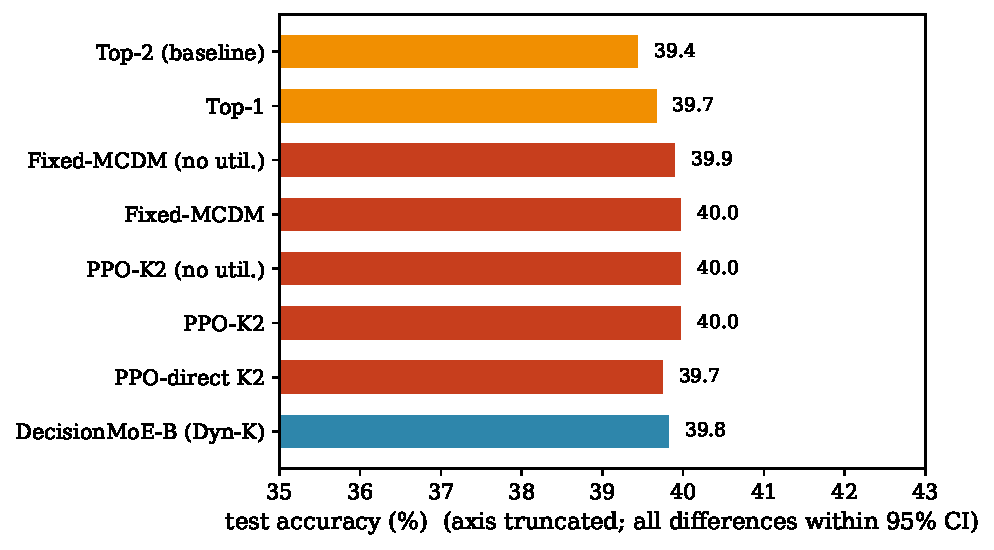
\includegraphics[width=\linewidth]{figures/f6_ablation.pdf}\caption{Test accuracy per variant.}\end{figure}
\begin{figure}[t]\centering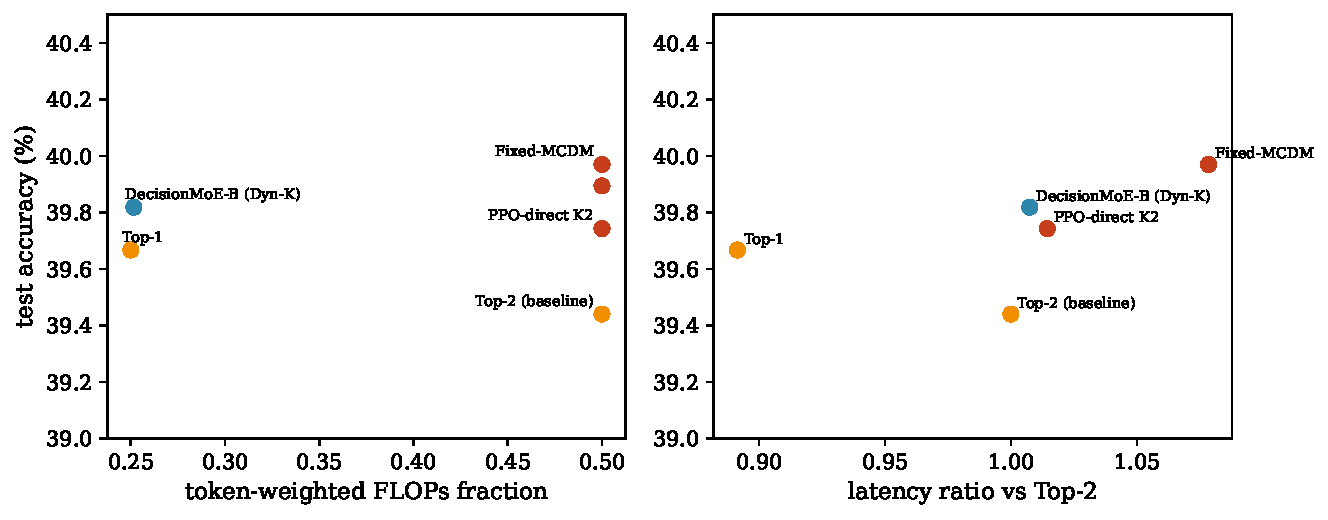
\includegraphics[width=\linewidth]{figures/f7_pareto.pdf}\caption{Accuracy vs. cost.}\end{figure}
\begin{figure}[t]\centering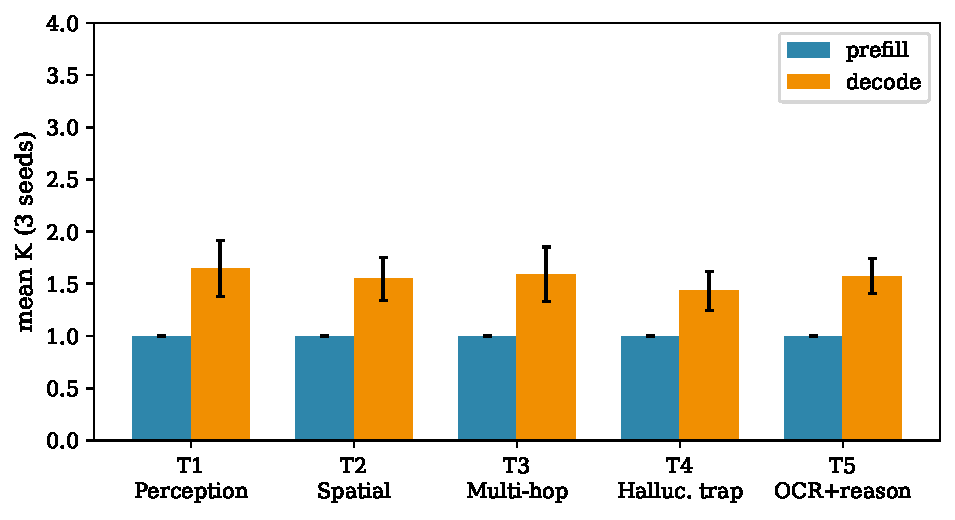
\includegraphics[width=.8\linewidth]{figures/f3_k_by_type.pdf}\caption{Mean $K$ by question type.}\end{figure}
\begin{figure}[t]\centering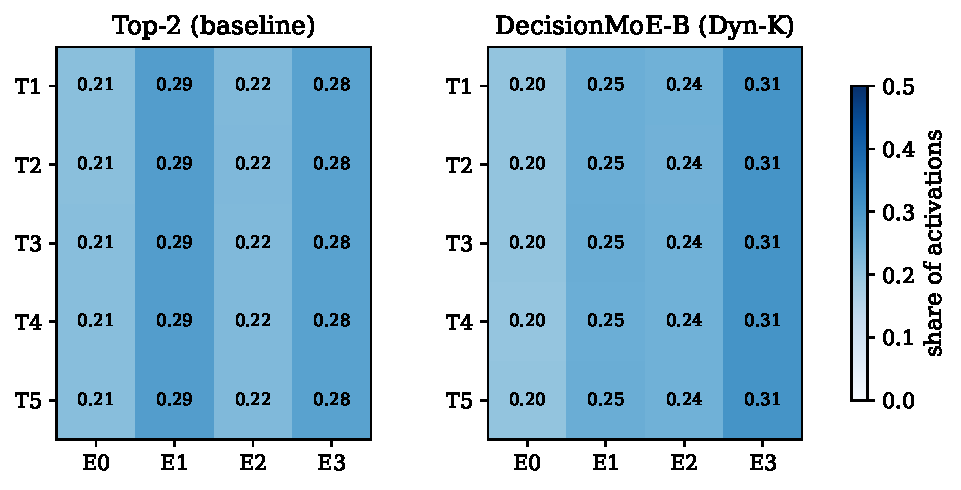
\includegraphics[width=\linewidth]{figures/f4_expert_by_type.pdf}\caption{Expert activation share by question type.}\end{figure}
\begin{figure}[t]\centering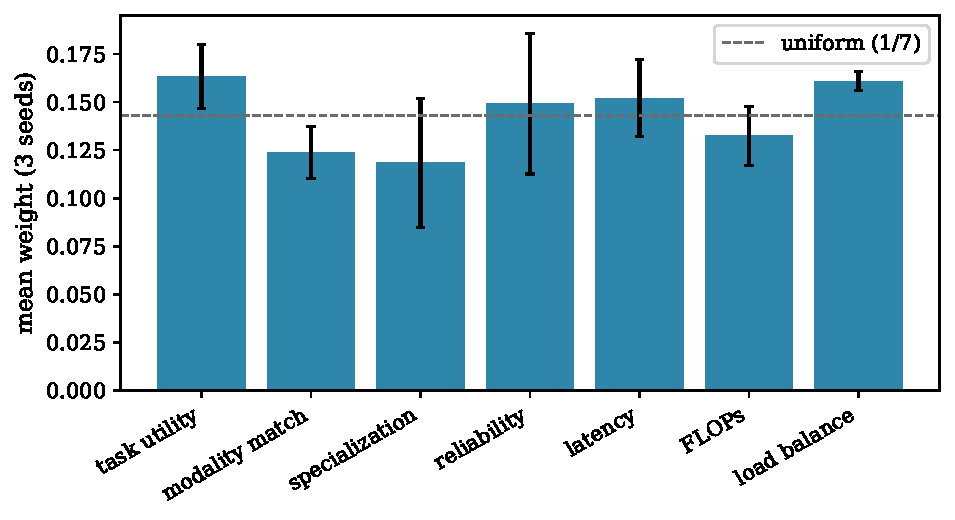
\includegraphics[width=.8\linewidth]{figures/f5_criteria_weights.pdf}\caption{Learned mean criterion weights.}\end{figure}
\subsection{Reward hacking}
\begin{figure}[t]\centering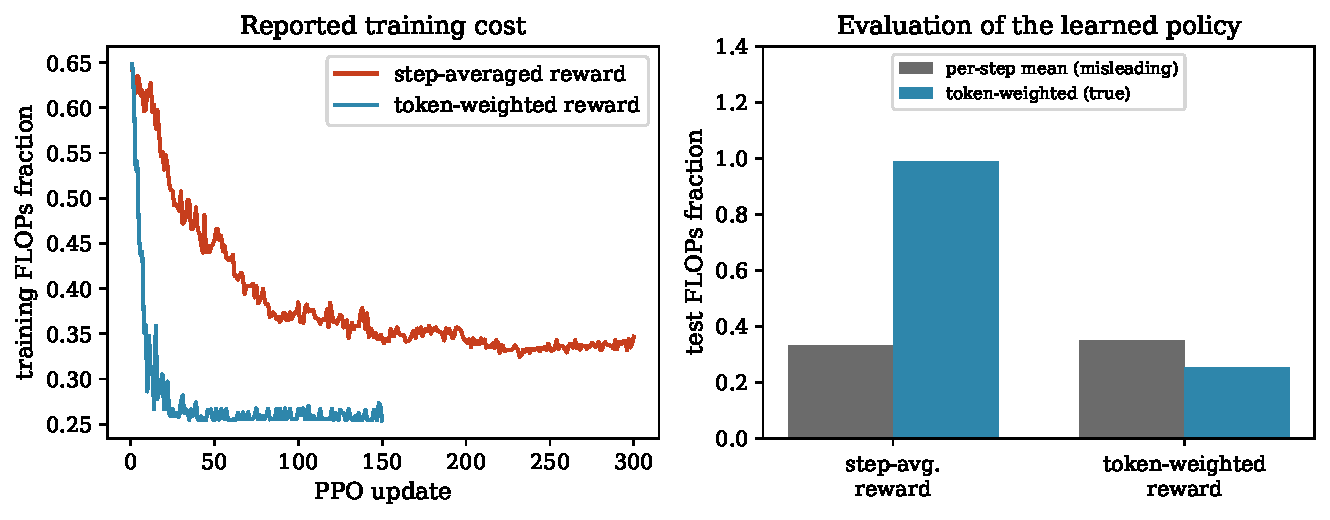
\includegraphics[width=\linewidth]{figures/f2_reward_hacking.pdf}\caption{Step-averaged vs. token-weighted FLOPs reward.}\end{figure}
\subsection{POPE}\begin{table}[t]
\centering
\small
\begin{tabular}{lccccccc}
\toprule
Method & Rand. & Pop. & Adv. & Acc. & F1 & $\bar K$ & $\Delta$ vs Top-2 \\
\midrule
Top-2 (baseline) & 87.2 & 85.8 & 83.9 & 85.6 & 83.9 & 2.00 & -- \\
Top-1 & 87.8 & 86.3 & 84.2 & 86.1 & 84.6 & 1.00 & +0.5 [+0.0, +0.9] \\
Fixed-MCDM & 87.7 & 86.0 & 84.5 & 86.1 & 84.4 & 2.00 & +0.4 [-0.0, +0.9] \\
PPO-direct K2 & 86.3 & 85.4 & 83.8 & 85.2 & 83.4 & 2.00 & -0.5 [-0.8, -0.2] \\
DecisionMoE-B (seed 42) & 86.4 & 85.3 & 83.2 & 85.0 & 83.1 & 1.51 & -0.7 [-1.2, -0.1] \\
DecisionMoE-B (seed 1) & 86.1 & 85.1 & 83.1 & 84.8 & 82.8 & 1.42 & -0.9 [-1.4, -0.4] \\
DecisionMoE-B (seed 2) & 85.8 & 84.9 & 83.0 & 84.6 & 82.5 & 1.50 & -1.1 [-1.6, -0.6] \\
\bottomrule
\end{tabular}
\caption{POPE (3$\times$1000 questions): accuracy per split, overall accuracy and F1 (\%), mean $K$, and paired accuracy difference vs. Top-2 (points, 95\% bootstrap CI). Learned Dynamic-K policies are slightly but consistently below the fixed baselines.}
\label{tab:pope}
\end{table}

\subsection{Manufactured specialisation}\begin{tabular}{lrrrcc}
\toprule
Model & $n$ & Top-2 & Oracle & Oracle$-$Top-2 (pp) & Right$-$wrong expert (pp) \\
\midrule
orijinal (n=400) & 400 & 0.450 & 0.445 & -0.5 [-2.2, +1.2] & -0.2 [-2.2, +1.7] \\
LoRA & 1074 & 0.485 & 0.496 & +1.1 [-1.2, +3.4] & +4.4 [+2.2, +6.8] \\
LoRA+kontrast & 1074 & 0.484 & 0.510 & +2.6 [+0.5, +4.8] & +5.5 [+3.5, +7.6] \\
LoRA+güçlü kontrast & 1074 & 0.496 & 0.505 & +0.8 [-1.5, +3.3] & +3.3 [+1.0, +5.5] \\
\bottomrule
\end{tabular}

\subsection{Second backbone: DeepSeek-VL2-Tiny}\begin{table}[t]\centering\small
\begin{tabular}{lccc}\toprule
Policy & FLOPs & Acc. & $\Delta$ vs Top-6 (pp)\\\midrule
topk-k6 & 1.000 & 0.471 & --\\
topk-k4 & 0.667 & 0.463 & -0.8 [-1.8,+0.3]\\
topk-k3 & 0.500 & 0.463 & -0.8 [-2.0,+0.3]\\
topk-k2 & 0.333 & 0.443 & -2.8 [-4.4,-1.2]\\
topk-k1 & 0.167 & 0.407 & -6.4 [-8.6,-4.2]\\
dyn-l005 & 0.667 & 0.466 & -0.5 [-1.5,+0.6]\\
dyn-l015 & 0.335 & 0.447 & -2.4 [-4.0,-0.8]\\
dyn-l040 & 0.168 & 0.413 & --\\
\bottomrule\end{tabular}
\caption{DeepSeek-VL2-Tiny on the synthetic test set (1,321 questions): accuracy and token-weighted expert FLOPs; $\Delta$ is the paired difference to Top-6 in points with 95\% CI.}
\label{tab:ds}
\end{table}
\begin{figure}[t]\centering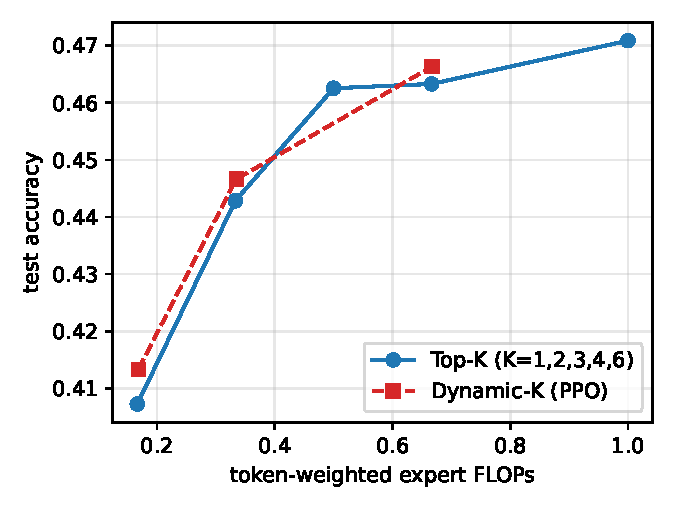
\includegraphics[width=.7\linewidth]{figures/f8_ds_pareto.pdf}\caption{DeepSeek-VL2-Tiny: accuracy vs. token-weighted expert FLOPs (test, 1,321 questions).}\end{figure}
\subsection{Long-generation regime: AI2D and ScienceQA-IMG}\begin{table}[t]\centering\small
\begin{tabular}{lcccc}\toprule
Policy & FLOPs & Acc. & Gain vs Top-K mix (pp) & Gain vs Top-K+static hull (pp)\\\midrule
\multicolumn{5}{l}{\textit{ai2d}}\\
topp0.5 & 0.449 & 0.533 & +3.3 [+0.2,+6.2] & +1.2 [-1.9,+4.2]\\
dyn-a020 & 0.338 & 0.462 & +0.0 [-1.7,+1.8] & -1.3 [-3.3,+0.7]\\
dyn-a040 & 0.344 & 0.486 & +2.1 [+0.3,+4.0] & +0.8 [-1.4,+2.9]\\
dyn-a080 & 0.199 & 0.369 & +2.6 [+0.6,+4.7] & +1.5 [-0.6,+3.6]\\
topp0.3 & 0.295 & 0.394 & -3.3 [-6.3,-0.3] & -4.4 [-7.5,-1.3]\\
topp0.4 & 0.395 & 0.461 & -2.1 [-4.7,+0.5] & -3.8 [-6.6,-1.1]\\
topp0.6 & 0.571 & 0.528 & -1.4 [-4.0,+1.3] & -3.1 [-6.2,-0.1]\\
topp0.7 & 0.683 & 0.566 & -1.2 [-3.9,+1.5] & -1.7 [-4.7,+1.3]\\
dyn-a040s1 & 0.344 & 0.484 & +2.0 [+0.1,+3.9] & +0.6 [-1.1,+2.4]\\
dyn-a040s2 & 0.338 & 0.476 & +1.4 [-0.4,+3.1] & +0.1 [-1.8,+1.9]\\
dyn-a080s1 & 0.171 & 0.320 & +0.3 [-1.1,+1.8] & -0.9 [-2.0,+0.3]\\
dyn-a080s2 & 0.171 & 0.322 & +0.5 [-0.9,+1.8] & -0.7 [-1.9,+0.4]\\
st1-4 & 0.170 & 0.328 & +1.2 [-0.2,+2.6] & +0.0 [+0.0,+0.0]\\
st2-3 & 0.336 & 0.469 & +0.8 [-0.9,+2.4] & -0.4 [-2.1,+1.2]\\
st2-4 & 0.339 & 0.476 & +1.3 [-0.4,+3.1] & +0.0 [+0.0,+0.0]\\
st2-5 & 0.341 & 0.469 & +0.6 [-1.1,+2.3] & -0.8 [-2.4,+0.9]\\
st3-4 & 0.505 & 0.534 & +1.5 [-1.2,+4.3] & -1.0 [-3.7,+1.8]\\
st3-5 & 0.510 & 0.546 & +2.5 [-0.2,+5.1] & +0.0 [+0.0,+0.0]\\
st2-6 & 0.344 & 0.474 & +1.0 [-0.9,+2.9] & -0.4 [-2.3,+1.6]\\
st3-3 & 0.500 & 0.518 & +0.0 [+0.0,+0.0] & -2.4 [-5.0,+0.3]\\
dyn-a040s3 & 0.338 & 0.482 & +2.0 [+0.1,+3.9] & +0.7 [-1.1,+2.6]\\
dyn-a040s4 & 0.486 & 0.514 & +0.2 [-2.6,+2.9] & -2.2 [-5.0,+0.7]\\
\multicolumn{5}{l}{\textit{sqa}}\\
dyn-a040 & 0.362 & 0.568 & -3.2 [-5.4,-1.0] & -3.8 [-7.4,-0.2]\\
dyn-a040s1 & 0.340 & 0.551 & -2.5 [-4.7,-0.2] & -3.1 [-6.9,+0.6]\\
dyn-a040s2 & 0.338 & 0.548 & -2.6 [-4.9,-0.3] & -3.2 [-7.0,+0.4]\\
dyn-a080 & 0.188 & 0.420 & +1.2 [-0.5,+3.0] & +0.4 [-1.2,+2.1]\\
topp0.5 & 0.447 & 0.693 & -0.2 [-3.3,+2.8] & -0.4 [-3.8,+2.9]\\
topp0.4 & 0.392 & 0.543 & -9.1 [-12.0,-6.3] & -9.6 [-13.4,-5.7]\\
topp0.6 & 0.568 & 0.760 & +0.5 [-1.7,+2.7] & -0.8 [-3.0,+1.4]\\
dyn-q040 & 0.495 & 0.786 & +3.5 [+1.6,+5.5] & +3.5 [+1.5,+5.5]\\
dyn-q040s1 & 0.502 & 0.765 & +1.0 [-0.7,+2.7] & +1.0 [-0.7,+2.6]\\
dyn-q040s2 & 0.401 & 0.727 & +8.2 [+5.7,+10.8] & +7.8 [+4.9,+10.7]\\
dyn-q040s3 & 0.390 & 0.719 & +8.7 [+6.0,+11.4] & +8.3 [+5.2,+11.3]\\
dyn-q040s4 & 0.430 & 0.745 & +6.9 [+4.3,+9.4] & +6.6 [+3.8,+9.4]\\
st1-4 & 0.173 & 0.400 & +0.8 [-0.5,+2.2] & +0.0 [+0.0,+0.0]\\
st2-3 & 0.338 & 0.556 & -1.7 [-3.8,+0.5] & -2.3 [-6.0,+1.4]\\
st2-4 & 0.342 & 0.534 & -4.3 [-6.6,-2.0] & -4.9 [-8.8,-1.1]\\
st2-5 & 0.345 & 0.528 & -5.4 [-7.7,-3.0] & -6.0 [-9.9,-2.1]\\
st3-4 & 0.505 & 0.747 & -0.8 [-3.0,+1.2] & -0.9 [-3.1,+1.2]\\
st3-5 & 0.509 & 0.754 & -0.2 [-2.3,+2.0] & -0.3 [-2.5,+1.8]\\
st2-6 & 0.349 & 0.536 & -5.0 [-7.3,-2.7] & -5.6 [-9.5,-1.8]\\
st3-3 & 0.500 & 0.755 & +0.0 [+0.0,+0.0] & +0.0 [+0.0,+0.0]\\
dyn-q020 & 0.502 & 0.757 & +0.2 [-1.9,+2.2] & +0.1 [-1.9,+2.1]\\
dyn-q080 & 0.406 & 0.737 & +8.7 [+6.2,+11.3] & +8.4 [+5.4,+11.3]\\
\multicolumn{5}{l}{\textit{aok}}\\
st1-4 & 0.169 & 0.471 & +0.9 [-0.3,+2.1] & +0.0 [+0.0,+0.0]\\
st2-3 & 0.337 & 0.640 & +0.6 [-1.5,+2.8] & +0.0 [+0.0,+0.0]\\
st2-4 & 0.340 & 0.626 & -0.8 [-3.1,+1.4] & -1.5 [-3.3,+0.4]\\
st3-3 & 0.500 & 0.720 & +0.0 [+0.0,+0.0] & +0.0 [+0.0,+0.0]\\
st3-4 & 0.502 & 0.715 & -0.4 [-1.9,+1.0] & -0.5 [-2.0,+1.0]\\
st3-5 & 0.504 & 0.715 & -0.4 [-2.0,+1.2] & -0.5 [-2.2,+1.1]\\
topp0.4 & 0.386 & 0.621 & -3.8 [-6.2,-1.4] & -4.3 [-6.7,-1.9]\\
topp0.5 & 0.450 & 0.695 & +0.1 [-2.0,+2.2] & -0.1 [-2.2,+2.1]\\
topp0.6 & 0.570 & 0.712 & +1.1 [-1.0,+3.1] & -0.9 [-3.0,+1.1]\\
dyn-o040 & 0.502 & 0.719 & -0.1 [-1.6,+1.4] & -0.2 [-1.7,+1.3]\\
dyn-o040s1 & 0.338 & 0.631 & -0.3 [-2.4,+1.8] & -0.9 [-2.9,+1.1]\\
dyn-o040s2 & 0.501 & 0.719 & -0.1 [-2.0,+1.7] & -0.2 [-2.0,+1.7]\\
dyn-o040s3 & 0.342 & 0.658 & +2.2 [-0.1,+4.6] & +1.6 [-0.6,+3.8]\\
dyn-o040s4 & 0.501 & 0.725 & +0.6 [-1.0,+2.0] & +0.5 [-1.0,+2.0]\\
\bottomrule\end{tabular}
\caption{AI2D and ScienceQA-IMG test sets (597 questions each): gain in accuracy points over the matched-FLOPs mixture of adjacent Top-K points, with paired-bootstrap 95\% CIs. PPO policies named a$\cdot$ were trained on AI2D, q$\cdot$ on ScienceQA.}\label{tab:mcq}
\end{table}
\begin{figure}[t]\centering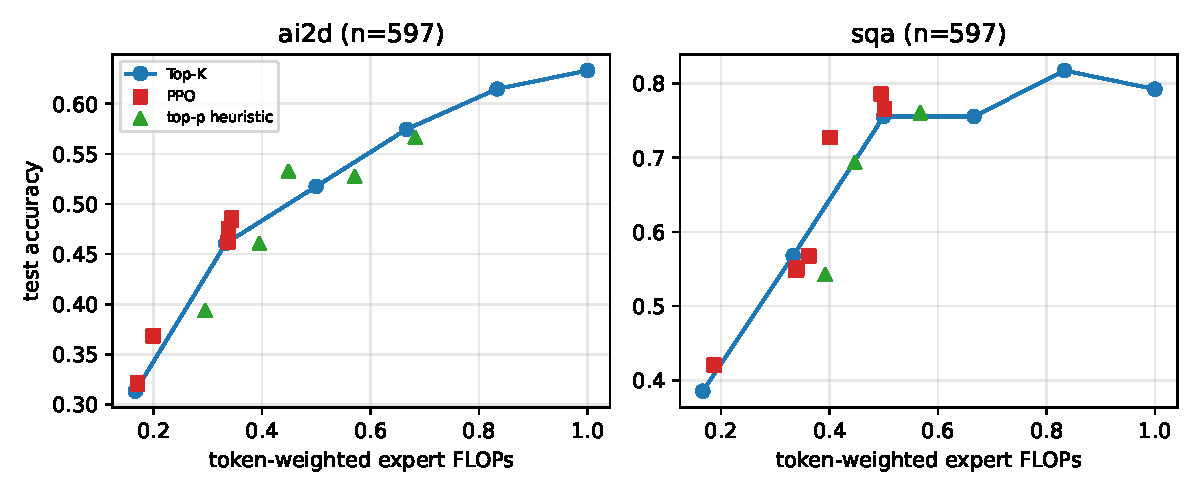
\includegraphics[width=\linewidth]{figures/f9_mcq_pareto.pdf}\caption{Accuracy vs. token-weighted expert FLOPs with brief chain-of-thought (test, 597 questions each).}\end{figure}
\bibliographystyle{plainnat}\bibliography{references}
\end{document}
